\documentclass[../../main.tex]{subfiles}

\graphicspath{{\subfix{images/}}}

\begin{document}

\chapter{Noțiuni Teoretice}
\label{ch:theory}

În acest capitol, vom prezenta \textbf{noțiunile teoretice necesare înțelegerii func\-ționării platformei propuse}. Concret, vom vorbi despre știința calculatoarelor pentru a avea contextul general al funcționării acestor dispozitive. Vom continua cu descrierea unor concepte de programe malițioase și de inteligență artificială, cu accent pe învățarea automată, urmând în finele capitolului să prezentăm succint noțiunile rămase, ce țin de funcționalitatea, arhitectura și implementarea platformei.

\section{Noțiuni Introductive}
\label{sec:theory_introduction}

Știința calculatoarelor reprezintă \textbf{studiul informației, a protocoalelor și a algoritmilor} folosiți pentru \textbf{automate reale și idealizate}. Ea cuprinde o serie de domenii, ce pot fi împărțite în \textbf{teoretice}, precum teoria computației, ce studiază modele și o serie de probleme ce pot fi rezolvate cu ajutorul lor, și \textbf{practice}, precum grafica ce analizează modele digitale de sintetizare și de manipulare a contextului grafic.

\subsection{Organizarea Internă a Calculatorului}

Modelul matematic prezentat de Alan Turing a reprezentat punctul de plecare al dezvoltării unor calculatoare digitale. În ciuda acestui fapt, în zilele noastre este folosită \textbf{arhitectura propusă de John von Neumann}, cunoscută sub numele de von Neumann sau Princeton. Aceasta cuprinde o serie de componente care face posibilă funcționarea oricărui calculator cu programe salvate, în care preluările de instrucțiuni și operațiile cu date nu pot apărea în același timp din cauza magistralei comune.

\begin{center}
    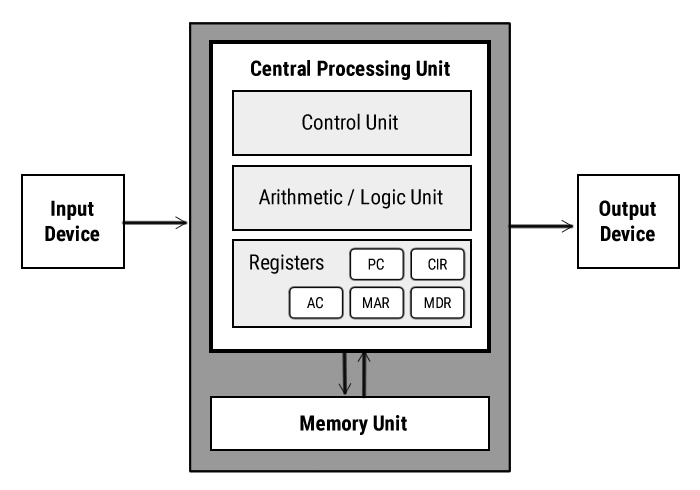
\includegraphics[width=7cm]{components/images/illustrations/vom_neumann_architecture.jpg}
    \label{fig:vom_neumann_architecture}
    \captionsetup{justification=centering,margin=1cm}
    \captionof{figure}[Arhitectura von Neumann a unui calculator]{Arhitectura von Neumann a unui calculator\footnotemark}
\end{center}
\vspace{0.3cm}

\footnotetext{\href{https://www.computerscience.gcse.guru/theory/von-neumann-architecture}{https://www.computerscience.gcse.guru/theory/von-neumann-architecture}}

Calculatorul poate fi privit ca având o \textbf{funcționare în trei etape}: intrarea datelor, procesarea și ieșirea datelor procesate. Astfel, prin intermediul unor dispozitive speciale, se preiau anumite stări sau acțiuni din mediul extern, în care calculatorul se află. Acestea sunt transportate prin intermediul unei magistrale către unitatea centrală, unde ele sunt procesate. Odată ce procesarea s-a finalizat, rezultatele sunt fie salvate în memoria volatilă ("\textit{random-access me\-mory}" și abreviat RAM), prin intermediul unității de gestiune a ei și pentru a fi utilizate ulterior pentru o altă procesare, fie întoarse în mediul exterior printr-o altă gamă de dispozitive speciale, de ieșire.

În arhitectura prezentată, \textbf{unitatea centrală de procesare} joacă cel mai important rol. Numită și procesor, este un circuit electronic construit în mare parte din tranzistori pe bază de silicon și capabil de a executa instrucțiunile ce formează un program. Multe procesoare sunt de natură sincronă, fapt ce implică un semnal de ceas pentru a impune un ritm operațiilor secvențiale executate. Semnalul este produs de un circuit oscilator extern, ce generează un număr constant de pulsuri electrice pe secundă.

\textbf{Ciclul de lucru al procesorului} presupune rularea în continuu a unei bucle formate din aducerea din memorie și decodificarea instrucțiunilor, aducerea din memorie a datelor necesare, execuția instrucțiunii și actualizarea opțională a memoriei. Cum de fiecare astfel de etapă se ocupă o unitate specializată a procesorului, o optimizare de tip linie de asamblare presupune \textbf{execuția para\-lelă a etapelor} astfel încât fiecare unitate să fie ocupată, în fiecare moment, cu procesarea unei instrucțiuni. În cel mai favorabil scenariu, acestă optimizare susține o rată de o instrucțiune pe fiecare ciclu de semnal de ceas.

\newpage

\subsection{Arhitecturi de Procesoare}

Abstractizarea modelului procesorului se realizează prin \textbf{arhitectura setului de instrucțiuni} ("\textit{instruction set arhitecture}" și abreviat ISA), definit de obicei ca "\textit{arhitectura procesorului}". Cum ISA oferă o interfață între hardware și software, sunt permise mai multe implementări ale ei, care pot varia în performanță, dimensiunea fizică și cost (timp, consum de energie electrică).

Cele mai uzuale arhitecturi pentru calculatoarele de uz general sunt ale companiilor Intel (în special IA-32 și IA-64) și Advanced Micro Devices. În același timp, Advanced RISC Machine sunt întâlnite pe dispozitive precum telefoane inteligente și tablete.

O astfel de arhitectură este definită, în general, de următoarele aspecte:
\begin{enumerate}
    \item \textbfit{Clasa}: Definește uzul operanzilor folosiți, putând fi cu regiștrii de uz general, unde operanzii pot fi regiștrii sau locații de memorie, sau de tip încărcare-stocare, în care memoria poate fi accesată numai prin instrucți\-uni speciale de lucru cu memoria.
    \item \textbfit{Adresarea memoriei}: Definește modul de interogare al memoriei, fiind de obicei la nivel de octet. Unele arhitecturi necesită ca obiectele din memorie să fie aliniate, adică adresa octetului de la care începe un astfel de obiect să fie divizibilă cu numărul de octeți pe care lucrează procesorul.
    \item \textbfit{Modelele de adresare}: Modelele de adresare sunt folosite la specificarea adreselor operanzilor. De obicei, aceștia pot fi regiștrii, valori constante sau deplasate, unde o valoare fixă, a zonei în care se află, este adăugată pentru a obține adresa de memorie reală.
    \item \textbfit{Operanzii}: Sunt descriși \textbf{de tip și de dimensiune}, acestea putând varia de la un octet (un caracter ASCII sau un \inlinecode{char}) și până la 8 octeți (\inlinecode{long integer}). Dimensiunea specifică arhitecturii este considerată ca fiind un \inlinecode{word}.
    \item \textbfit{Operațiunile}: Operațiunile sunt împărțite în categorii, cele mai uzuale fiind de transfer de date, logice, aritmetice, de control și de lucru cu numere reale.
    \item \textbfit{Instrucțiunile de control ale execuției programului}: Obligatorii pentru toate arhitecturile, sunt cele de salturi condiționale sau necondițio\-nale, apeluri de proceduri și întoarcere la funcția apelantă.
    \item \textbfit{Codificarea ISA}: Poate fi realizată în două maniere: una în care lungimea instrucțiunilor este fixă și una în care aceasta este variabilă. Ultima abordare dispune de avantajul de a avea o relație de proporționalitate directă între dimensiunea instrucțiunii și raritatea ei (cu cât o instrucțiune este statistic folosită mai mult, cu cât lungimea de codificare este mai mică). Astfel, codificarea ISA definește modul în care instrucțiunile sunt reprezentate în memorie, ca și coduri de operație formate dintr-un grup de biți, ce specifică operațiunea ce se dorește a fi executată, și un altul, ce indică informații suplimentare necesare operației, precum operanzii acesteia.
\end{enumerate}

\subsubsection{Regiștrii}

Zonele de memorie interne ale procesorului sunt numite \textbf{regiștrii}. Comparativ cu alte tipuri de memorii (cache, RAM, disc) aflate la dispoziția procesorului, ei au o viteză de manipulare foarte mare, de ordinul nanosecundelor. Acest avantaj vine însă la pachet cu dezavantaje, ei fiind puțini și de o lungime mică, dictată de ISA.

Cei mai uzuali regiștrii pot fi grupați în funcție de scopul lor, astfel:
\begin{itemize}
    \item \textbf{Uz general}, care salvează operanzi și rezultate ale diverselor operații;
    \item \textbf{Starea programului} și \textbf{control} (limitat) al procesorului; și
    \item \textbf{Salvarea adresei instrucțiunii} ce urmează să fie executată.
\end{itemize}

\subsubsection{Memorie Virtuală. Paginare. Segmentare}

O problematică luată în considerare de arhitecții de procesoare reprezintă spațiul prea mare ocupat de mai multe procese (o astfel de entitate poate fi privită ca un program aflat în execuție la un anumit moment de timp), în condițiile în care acestea ocupă numai o mică parte din spațiul lor de adrese. Soluția găsită a fost \textbf{memoria virtuală}, ce împarte memoria RAM în blocuri, pe care le alocă diferitelor procese în funcție de nevoile lor. Aceste blocuri pot fi mutate pe disc în cazul în care sunt folosite rar, ele fiind aduse în memoria principală numai atunci când sunt accesate.

Mecanismul ce oferă suportul memoriei virtuale dispune de două tehnici: una ce lucrează cu blocuri de lungime fixă, numite \textbf{pagini}, și una cu blocuri de lungimi variabile, numite \textbf{segmente}. Decizia de a folosi o tehnică în favoarea alteia influențează viteza cu care procesorul funcționează, prin considerarea unor factori precum:
\begin{itemize}
    \item Lungimea adresei, în \inlinecode{word}-uri, cu unul pentru pagini și două (identificatorul segmentului și deplasarea în segment) pentru segmente;
    \item Dificultatea înlocuirii unui bloc, fiind trivial pentru pagini datorită lungi\-mii constante și dificil pentru segmente deoarece trebuie găsită o zonă continuă de memorie, neocupată; și
    \item Ineficiența folosirii memoriei, cu fragmentare internă pentru pagini și externă pentru segmente.
\end{itemize}

\subsection{Limbaj de Asamblare}

În funcție de abstractizarea dorită, se pot apela mai multe niveluri pentru a programa un procesor să execute o sarcină dată. Aceste niveluri formează o stivă, ce este ilustrată în figura de mai jos.

\begin{center}
    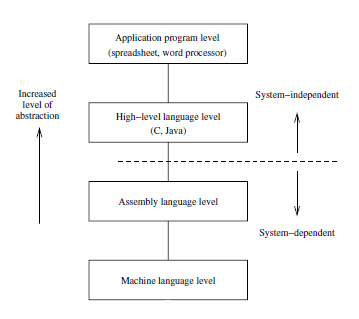
\includegraphics[width=7cm]{components/images/illustrations/abstraction_levels.png}
    \label{fig:abstraction_levels}
    \captionsetup{justification=centering,margin=1cm}
    \captionof{figure}[Niveluri de interacțiune cu un sistem de calcul]{Niveluri de interacțiune cu un sistem de calcul\footnotemark}
\end{center}
\vspace{0.3cm}

\footnotetext{\fullcite{assembly_intro}}

Cele mai înalte două niveluri limitează utilizatorul fie la lucrul cu o aplicație, fie la programarea într-un limbaj de nivel superior, pentru a-și scrie aplicații de unul singur. În ambele cazuri, nu este o necesară o cunoaștere detaliată a sistemului datorită independenței acestora două (de exemplu, de un procesor particular, utilizat în cadrul sistemului), excepție făcând cazul în care dezvoltarea implică noțiuni mai avansate, de exemplu de drivere. Pe de altă parte, limbajul de asamblare și cel mașină sunt de nivel inferior. Instrucțiunile lor permit realizarea unor sarcini de nivel mai jos comparativ cu cele menționate anterior.

\textbf{Limbajul de asamblare} reprezintă un mod de a afișa limbajul mașină, ce reprezintă numai o înșiruire de octeți ce pot fi înțeleși de către procesor. Pentru a realiza traducerea, limbajul de asamblare trebuie procesat de către un program numit \textbf{asamblor}.

Este format din instrucțiuni ce trebuie să respecte un anumit format, și anume \inlinecode{eticheta: mnemonic argumente}. Eticheta reprezintă o notație prin care alte instrucțiuni, precum cele de salt, pot face referire la instrucțiunea curentă. Mnemonicul este un nume rezervat pentru o clasă de instrucțiuni care au aceeași funcționalitate. Operanzii, având un număr variabil în funcție de codul operației, sunt folosiți pentru a executa instrucțiunea.

\vspace{0.3cm}
\begin{center}
    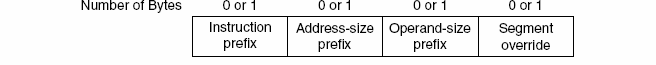
\includegraphics[width=10cm]{components/images/illustrations/x86_instruction_format.png}
    \label{fig:x86_instruction_format}
    \captionsetup{justification=centering,margin=1cm}
    \captionof{figure}[Structura unei instrucțiuni pe arhitectura x86]{Structura unei instrucțiuni pe arhitectura x86\footnotemark}
\end{center}

\footnotetext{\href{http://www.c-jump.com/CIS77/CPU/x86/lecture.html}{http://www.c-jump.com/CIS77/CPU/x86/lecture.html}}

Deși programele dezvoltate în limbajul de asamblare au avantajul de a rula cu o viteză foarte mare pe procesoarele țintă, datorită folosirii optime a resurselor pe care acestea le oferă, ele sunt greu de dezvoltat, de întreținut și sunt dependente de ISA. Din aceste motive, s-a introdus un nivel nou care să îmbunătățească interfață cu resursele fizice ale calculatorului și să reducă timpul dezvoltării programelor: sistemul de operare

\subsection{Sisteme de Operare}

\textbf{Sistemele de operare} sunt sisteme de programe care oferă programatorilor o interfață simplă prin care să lucreze cu componentele complexe ale calculatorului, pe care le are în gestiune.

Fiind un software fundamental, sistemul de operare rulează într-un mod privilegiat, numit mod nucleu, în care are acces deplin la hardware și poate executa orice instrucțiune de care calculatorul e capabil. Pe de altă parte, celelalte programe rulează în modul utilizator, în care drepturile sunt limitate.

\subsubsection{Procese și Fire de Execuție}

Un program din modul utilizator, aflat în execuție, se numește \textbf{proces}. Asociat fiecărui proces este un \textbf{spațiu de adrese}, adică o zonă de memorie în care programul poate să scrie și să citească și care conține zone dedicate pentru programul executabil, datele programului, stiva acestuia. Pe lângă cele menționate, mai include regiștrii salvați ai procesorului, o listă de fișiere deschide, procese înrudite și alte informații necesare execuției.

Sistemele de operare moderne permit, prin intermediul unui concept numit \textbf{multiprogramare} (engl. "\textit{multitasking}"), rularea a mai multor procese în același timp, cu condiția ca numai un număr fix (egal cu numărul de procesoare al calculatorului) să se afle în execuție. În acest timp, restul proceselor se află într-o stare de suspendare temporară, datele lor fiind salvate într-un \textbf{tabel de procese}, ce este un vector de structuri specifice (engl. "\textit{process control block}"), una pentru fiecare proces. După o anumită cuantă de timp, stabilită de un proces dedicat numit \textbf{planificator}, procesele aflate în execuție sunt întrerupte, iar o altă serie de procese încep să fie executate.

\begin{center}
    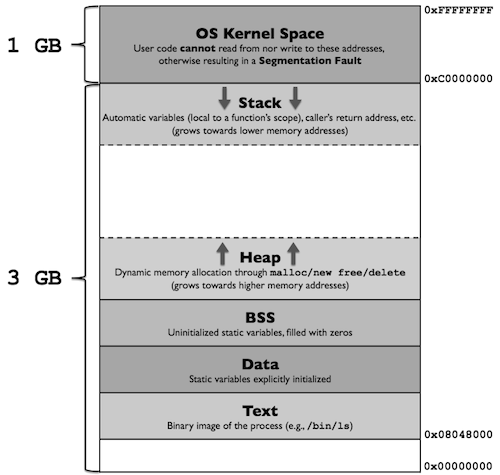
\includegraphics[width=7cm]{components/images/illustrations/memory_layout.png}
    \label{fig:memory_layout}
    \captionsetup{justification=centering,margin=1cm}
    \captionof{figure}[Organizarea spațiului de adrese al unui proces]{Organizarea spațiului de adrese al unui proces\footnotemark}
\end{center}
\vspace{0.3cm}

\footnotetext{\href{https://gabrieletolomei.wordpress.com/miscellanea/operating-systems/in-memory-layout}{https://gabrieletolomei.wordpress.com/miscellanea/operating-systems/in-memory-layout}}

Fiecare proces își poate defini în cadrul său mai multe \textbf{fire de execuție}, cărora li se poate aloca timp de procesor de către planificator. Aceste entități împărtășesc același spațiu de adrese cu procesul care le-a creat, diferența fiind pentru stivă și pentru variabilele statice, ce sunt specifice și salvate într-un spațiu dedicat, local firului. Toate aceste spații aparțin de un bloc de mediu (engl. "\textit{thread environment block}").

\subsubsection{Apeluri de Sistem}

Sistemul de operare expune programelor din spațiul utilizator o serie de funcțio\-nalități, ce vor fi executate cu privilegii depline, adică în modul privilegiat. Aceste \textbf{apeluri de sistem} se află în evidența sistemului de operare fie prin metode exportate de către o librărie, precum \inlinecode{ntdll.dll} de pe sistemele de operare Windows, fie printr-un index într-o tabelă, cum este cazul în sistemele de operare UNIX.

Pentru invocarea unui apel de sistem, procesul trebuie să pregătească datele ce vor fi transmise și să creeze o cerere de întrerupere, pentru a ceda contextul rutinei privilegiate. După ce aceasta se execută, va salva rezultatul într-o locație uzuală (registru sau zonă de memorie dată ca argument), va restabili contextul și va reda dreptul de execuție procesului apelant.

\newpage

\subsection{Sisteme de Fișiere}

Asemenea procesoarelor ce sunt abstractizate sub formă de procese, memoria este tratată în aceeași manieră. Ea este modelată de către sistemul de operare sub formă de \textbf{fișiere}, unități logice de informație create de procese. Această abordare are o serie de avantaje:
\begin{itemize}
    \item Dimensiunea mare a informației ce poate fi stocată;
    \item Persistența informației, chiar și după terminarea procesului; și
    \item Concurența accesării informației, de către mai multe procese.
\end{itemize}

Toate fișierele sunt gestionate printr-o metodologie specifică, ce stabilește cum sunt structurate, accesate, modificate și protejate fișierele și ce este implementată într-o componentă a sistemului de operare numită \textbf{sistem de fișiere}.

\subsubsection{Fișiere}

\textbf{Fișierele} sunt cea mai mică unitate care permite salvarea persistentă de date.

Acestea sunt create și ulterior identificate de către procese prin intermediul unui \textbf{nume} ce conține o secvență dintr-un set de caractere, diferit de la o implementare la alta. În unele sisteme de fișiere, numele sunt compuse din două părți, separate prin punct. În timp ce prima identifică fișierul, \textbf{extensia} (cea de-a doua parte) indică anumite caracteristici ale fișierului, caracteristici ce pot fi folosite pentru procesarea lui.

În cazul în care extensia nu este prezentă, sistemele de operare precum cele UNIX se folosesc de o serie de octeți din antet, numită \textbf{număr magic} (engl. "\textit{magic number}"), pentru a identifica tipul fișierului.

Pe lângă nume și date, sistemele de operare mai asociază fișierelor date suplimentare, numite \textbf{atribute}. Acestea pot oferi informații utile, precum timpul creării sau a ultimei modificări a fișierului, dimensiunea și drepturi necesare pentru a efectua diverse operații asupra sa.

Cele mai întâlnite operații asupra fișierelor, în sistemele de operare mo\-derne, sunt: creare, redenumire, ștergere, deschidere, închidere, citire, scriere și modificarea atributelor.

\subsubsection{Directoare}

Fișierele descrise anterior sunt salvate, de regulă, în interiorul unor \textbf{directoare}. Acestea sunt o formă specială de fișiere, identificate prin nume, care pot avea copii sub forma unor referințe către alte fișiere. În acest fel, se construiește o structură arborescentă.

Pentru a prelua numele unui nod dintr-o astfel de structură, sunt disponibile două abordări: una \textbf{absolută}, în care se efectuează o parcurgere de la \textbf{directorul rădăcina} și până la nodul de interes, și una \textbf{relativă}, față de \textbf{directorul curent}.

Operații uzuale asupra directoarelor sunt: creare, redenumire, ștergere, des\-chidere, închidere, referențiere (prin care fișiere poate apărea în două directoare în același timp) și dereferențiere.

\subsection{Fișiere Executabile}

Atunci când sistemul de operare dorește să creeze un proces nou (din motive precum apeluri de sistem din cadrul altor procese, comenzi ale utilizatorului sau sarcini periodice), se folosește o componentă specială de încărcare (engl. "\textit{loader}") pentru a pleca de la un \textbf{fișier de tip executabil}. După alte câteva operațiuni, printre care identificarea anumitor zone de memorie și popularea stării inițiale, procesul este rulat plecând de la un anumit punct, indicat în fișier printr-un câmp numit \textbf{punct de intrare} (engl. "\textit{entry point}").

În același timp, fișierul executabil se poate folosi de resurse externe, non-volatile, ce pot fi împărtășite de către mai multe programe și ce sunt numite \textbf{biblioteci}. Acestea conțin implementări ale unor comportamente predefinite, ce pot fi legate în două maniere. \textbf{Legarea statică} presupune copierea directă a lor în fișierul executabil final, în timp ce \textbf{legarea dinamică} doar referențiază acele implementări, urmând ca la încărcarea în memorie a programului să fie încărcate și acele librării, pentru a putea apela funcționalitățile ei.

\subsubsection{Divizarea Spațiului de Adrese}

Spațiul de adrese folosit de către un program este divizat în mai multe \textbf{segmente}, fiecare cu o funcționalitate diferită. Acestea sunt identificate prin etichete, ce apar și în limbajul de asamblare, pe baza căruia executabilul este format.

Segmentul de \textbf{cod}, având eticheta \inlinecode{.code}, conține codul mașină rezultat în urma compilării codului sursă al programului. Este de obicei protejat împotriva scrierii pentru a asigura anumite cazuri în care acest segment este suprascris neintenționat (din cauza unei referințe neinițializat corect) sau intenționat (în programe împachetate).

Segmentele de \textbf{date} conțin variabile globale, statice, constante sau externe. Acestea pot fi inițializate, caz în care segmentul are eticheta \inlinecode{.data}, sau neinițiali\-zate, într-un segment cu eticheta \inlinecode{.bss}. Pe de altă parte, segmentul de \textbfit{heap} conține variabilele alocate dinamic, de exemplu prin apelul funcției \inlinecode{malloc}, specifice limbajului de operare C, din librăria \inlinecode{stdlib.h}.

Segmentul de \textbf{stivă} salvează, pe lângă argumentele programului, adresa de întoarcere (următoarea instrucțiune a funcției apelante, după apelul funcției curente), vechea referință către baza stivei, argumentele și variabilele locale. Toate acestea sunt grupate într-o zonă continuă de memorie numită \textbf{cadru} și identificată prin două referințe, unul către bază și unul către vârf.

Modul în care se gestionează stiva este numit \textbf{convenție de apelare} și este restricționat fie de către ISA, fie de către compilatorul cu care fișierele executabile se creează. Această convenție conține detalii precum modul în care se transmit parametrii de la funcția apelantă la cea apelată, locația în care se salvează valoarea de retur și funcția care restaurează stivă.

\subsubsection{Portable Executable}

Un format de fișiere reprezentativ pentru cele executabile, obiect și librării dinamice este \textbf{Portable Executable}, prezent pe sistemele de operare Windows.

Pentru formatul executabil, \textbf{antetul} începe cu un șir de octeți, specifici antetului de Microsoft Disk Operating System și păstrați datorită dorinței de compatibilitate. Este urmat de o semnătură de 4 octeți (\inlinecode{PE0\textbackslash0\textbackslash0}) și alte informații esențiale rulării programului, precum:
\begin{itemize}
    \item Dimensiunea secțiunilor;
    \item Dimensiunile maxime ale secțiunilor de stivă și de \textit{heap};
    \item Adresa punctului de intrare, relativă la adresa de bază; și
    \item Subsistemul folosit.
\end{itemize}

După acestea, urmează un tabel, în care fiecare intrare reprezintă un antet al unei secțiuni, cu detalii precum dimensiunile fizice, virtuale și caracteristicile (o serie de biți ce indică anumite proprietăți ale secțiunii, printre care alinierea și drepturile asupra ei), și secțiunile fișierului executabil.

\vspace{0.3cm}
\begin{center}
    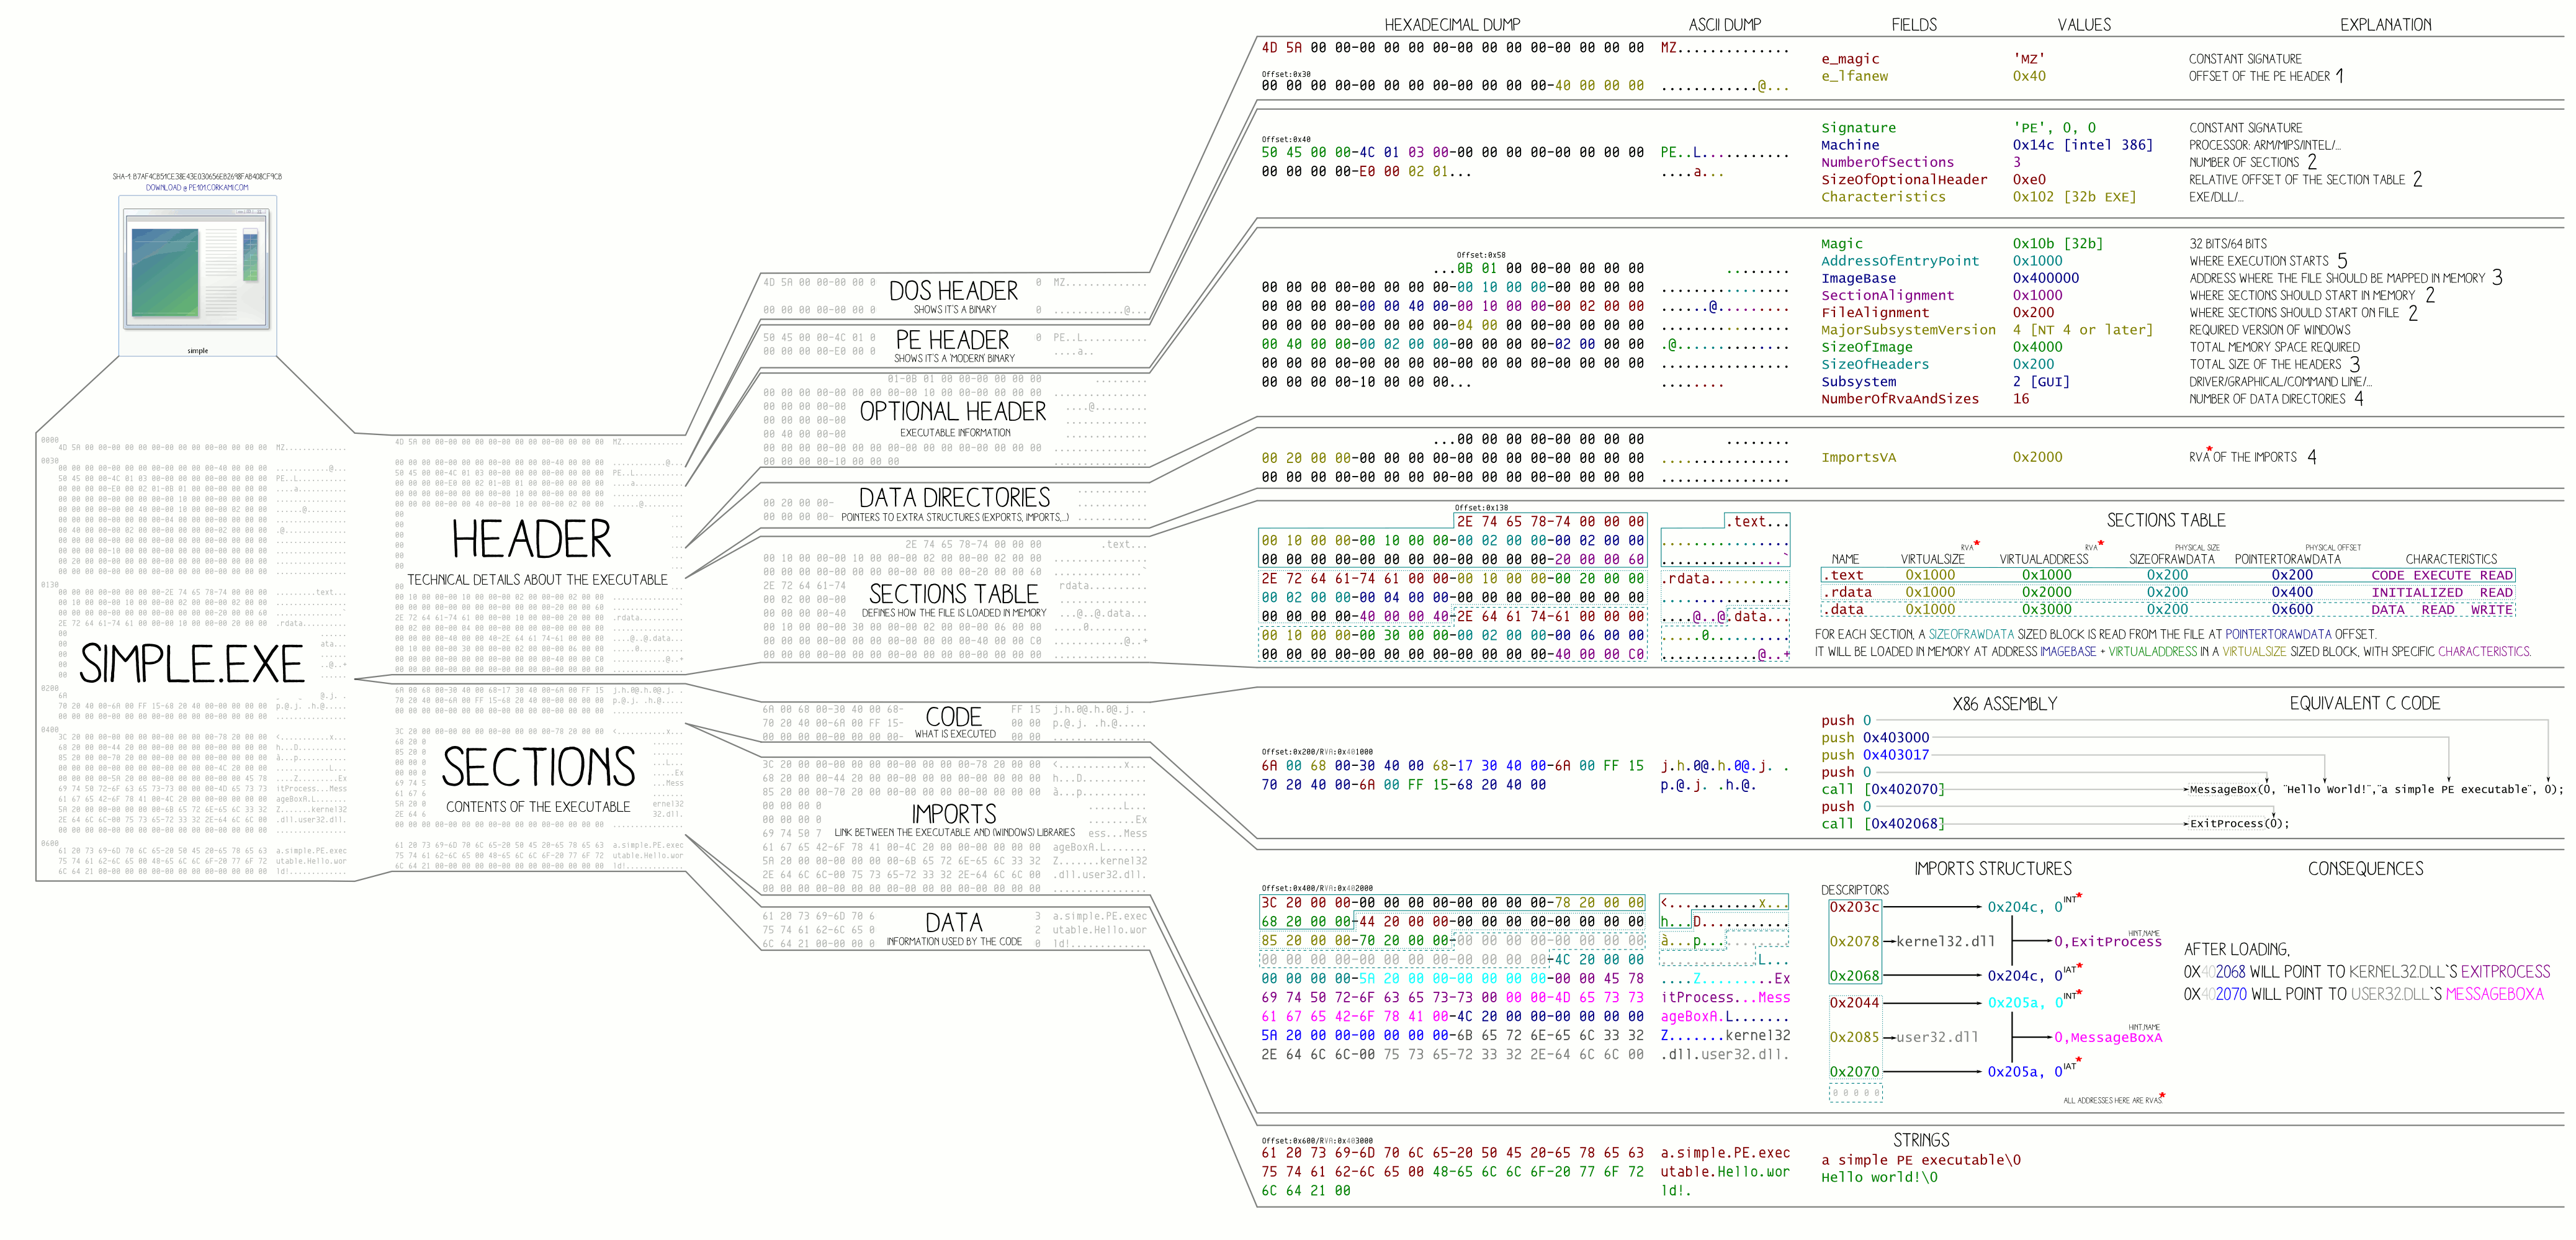
\includegraphics[width=10cm]{components/images/illustrations/pe.png}
    \label{fig:pe}
    \captionsetup{justification=centering,margin=1cm}
    \captionof{figure}[Structura formatului Portable Executable]{Structura formatului Portable Executable\footnotemark}
\end{center}
\vspace{0.3cm}

\footnotetext{\href{https://github.com/corkami/pics/blob/master/binary/pe101/pe101l.png}{https://github.com/corkami/pics/blob/master/binary/pe101/pe101l.png}}

\subsubsection{Fișiere OLE}

Formatul OLE, al cărui nume provine din abrevierea sintagmei din limba engleză "\textit{Object Linking and Embedding}", este o tehnologie proprietară companiei Microsoft care permite încorporarea și referențierea de obiecte în cadrul unor fișiere compuse. De regulă, este utilizat în \textbf{suita de programe Microsoft Office}, pentru documente, prezentări, tabele de calcul și baze de date, și în mesajele Outlook.

Sunt disponibile două formate diferite OLE, și anume \inlinecode{1.0} și \inlinecode{2.0}. Ultimul este cel recomandat pentru a fi folosit când se creează documente de tip container\footnote{\href{https://docs.microsoft.com/en-us/openspecs/windows_protocols/ms-oleds/fdc5e702-d09e-4344-a77f-eb079d41f23f}{https://docs.microsoft.com/en-us/openspecs/windows\_protocols/ms-oleds/fdc5e702-d09e-4344-a77f-eb079d41f23f}}, versiunea \inlinecode{1.0} fiind suportată de programele actuale numai pentru compatibilitate.

Fiind un obiect compozit, un fișier în format OLE este compus din:

\begin{itemize}
    \item \textbfit{Fluxuri de date} (engl. "\textit{streams}"): Sunt asemănătoare unor fișiere incluse într-o arhivă. Fiecare este identificat printr-un nume, de exemplu fluxul \inlinecode{WordDocument} dintr-un fișier Microsoft Word care conține textul său.
    \item \textbfit{Depozite} (engl. "\textit{storages}"): Sunt grupări de fluxuri de date sau de alte depozite. Un exemplu de depozit este cel identificat prin numele \inlinecode{Macro}, ce conține acele secvențe de cod Visual Basic for Applications (abreviat VBA) folosite pentru automatizarea conținutului documentului.
    \item \textbfit{Proprietăți}: O proprietate este o valoare ce poate fi folosită la stocarea unei informații relevante, precum date despre documentul curent (titlu, autor, date de creare și modificare).
\end{itemize}

\subsection{Comunicații în Rețea}

Deși unele programe executabile sunt concepute pentru a rula pe un singur sistem de calcul, intervin situații în care este necesară o conexiune a mai multor astfel de sisteme. Acestă comunicație dintre ele, numită \textbf{rețea}, presupune trimiterea unor \textbf{pachete} cu date, date din cele ale resursei ce se dorește a fi partajată. În același timp, emițătorul și receptorul respectă un set comun de reguli, definit într-un \textbf{protocol}.

În proiectarea modernă, protocoalele de rețea sunt stratificate pentru a forma o \textbf{stivă}. Cea mai cunoscută este \textbf{stiva TCP/IP}, în care pe straturile de rețea și de transport apar protocoalele Internet Protocol (abreviat IP), respectiv Transmission Control Protocol (abreviat TCP). Tot sistemul global de dispozitive interconectate ce folosesc această suită de protocoale formează \textbf{Internetul}.

\section{Aplicații Malițioase}
\label{sec:theory_malware}

Orice aplicație care este proiectată în mod intenționat pentru a provoca un prejudiciu unui utilizator, unui calculator sau unei rețele de calculatoare se numește \textbf{aplicație malițioasă} (engl. "\textit{malware}").

\subsection{Tehnici, Tactici și Proceduri}

De regulă, aplicațiile malițioase urmăresc un șablon comun. Primul pas surprinde momentul în care un utilizator face o acțiune ce provoacă descărcarea programului. Această acțiune poate consta în vizitarea unei pagini web malițioase, descărcarea unui atașament dintr-un email, a unui fișier dintr-o rețea de partajare sau conectarea unui stick USB cu un software (engl. "\textit{firmware}") adaptat de către atacator. Odată ce aplicația malițioasă a fost rulată după descărcare, ea infectează calculatorul și începe să lucreze pentru îndeplinirea scopurilor creatorului.

Deși comportamentul acestor programe este diferit de la un exemplar la altul, s-a efectuat o standardizare prin intermediul \textbf{tacticilor, tehnicilor și procedurilor} (engl. "\textit{tactics, techniques and procedures}" și abreviat TTP). Tacticile reprezintă motivul pentru care actorul efectuează acea acțiune malițioasă. Tehnicile, pe de altă parte, sunt modalitatea prin care obiectivul tactic este îndeplinit, în timp ce procedurile sunt implementări specifice ale programului malițios, utilizate în cadrul tehnicii.

Un \textit{framework} public de cunoștințe despre programe malițioase, cu observații din lumea reală, este MITRE ATT\&CK\footnote{\href{https://attack.mitre.org}{https://attack.mitre.org}}. Conține matrice în care TTP-urile sunt grupate, permițând astfel analiștilor și organizațiilor să înțeleagă mai bine amenințările de care se lovesc.

\subsection{Actori}

Aplicațiile malițioase sunt realizate de către \textbf{actori}, ce pot fi clasificați în funcție de scopul efectuării unei astfel de activități prejudicioase:
\begin{itemize}
    \item \textbfit{Criminalii cibernetici}: Reprezintă acele persoane care urmăresc obține\-rea de profit și de reputație, formând cea mai întâlnită categorie de actori. Ei pot fi individuali sau parte dintr-o echipă mai mare. Principalele tehnici folosite de ei sunt atacurile de tip \textit{phishing} (obținerea de informații senzitive prin deghizarea sub o entitate de încredere), ingineria socială, atacul prin forță brută al parolelor și \textit{ransomware}.
    \item \textbfit{Persoanele din interior}: Sunt angajați, contractori sau parteneri ai unei companii, care au acces la rețeaua, sistemele și date corporative. Dorința lor de a provoca daune companiei țintă se motivează prin dorința de a avea câștiguri financiare sau prin căutarea răzbunării. Se folosesc de tehnici precum exfiltrarea de date și abuzarea privilegiilor deținute.
    \item \textbfit{Actorii statali}: Pot fi parte din organizația internă a unui stat sau pot primi direcții, finanțare și asistență tehnică de la state. Ei atacă și obțin persistență în sectoarele publice și private cu scopul de a fura, schimba sau distruge informație. Cele mai întâlnite tehnici sunt atacurile de tip \textit{spear-phishing} (atac de tip \textit{phishing}, vizat unui anumit individ sau unei organizații anume), ingineria socială și accesul de la distanță prin programe de tip \textit{backdoor}.
    \item \textbfit{Hacktivists}: Cuprinde acei actori ce sunt motivați politic, social sau ideologic și ce întreprind acțiuni ilegale, malițioase pentru obținerea vizi\-bilității sau a unor schimbări în ariile în care ei activează. Folosesc tehnici precum atacurile de întrerupere distribuită a serviciilor (engl. "\textit{distributed denial of service}"), \textit{doxing} (identificarea și publicarea online a unor informații) și vandalizarea website-urilor (engl. "\textit{website defacement}").
    \item \textbfit{Organizațiile teroriste}: Folosesc acțiuni ofensive cu scopul de a obține câștiguri materiale, de a spiona sau de face propagandă. Tehnicile folosite sunt deteriorarea website-urilor și publicarea de informații false.
\end{itemize}

\subsection{Taxonomia Programelor Malițioase}

O clasificare mai grosieră decât cea prin atribuirea de TTP-uri constă în identificarea comportamentului unitar al programului malițios. Cum majoritatea programelor de acest tip cad într-una din aceste categorii, abordarea de față poate ajuta la efectuarea analizei prin stabilirea unei ipoteze ce poate fi confirmată sau infirmată în urma unei analize mai amănunțite:
\begin{itemize}
    \item \textbfit{Backdoor}: Sunt programe ce se instalează singure, fără interacțiunea specifică a utilizatorului și cu scopul de a oferi atacatorilor acces și posibilitatea de a executa comenzi.
    \item \textbfit{Botnet}: Reprezintă un program prin care sistemele compromise primesc toate aceeași comandă de la atacator, prin intermediul unui server de comandă și control.
    \item \textbfit{Downloader}: Permite numai descărcarea și instalarea altui program malițios.
    \item \textbfit{Spyware}: Colectează informații de pe calculatorul infectat și le trimite către atacator.
    \item \textbfit{Rootkit}: Sunt programele specializate în ascunderea existenței altor programe malițioase pe sistemul local, de regulă față de programele de tip antivirus.
    \item \textbfit{Scareware}: Au scopul de a determina proprietarul sistemului infectat să cumpere anumite servicii, cu unicul obiectiv de a îmbunătăți situația financiară a atacatorului.
    \item \textbfit{Virușii} (sau programe de tip \textbfit{worm}): Se propagă în rețea, infectând calculatoarele conectate între ele.
\end{itemize}

\subsection{Indicatori de Compromitere}

\textbf{Indicatorii de compromitere} reprezintă o evidență obținută din urma unei analize, care indică o posibilă infecție a unui sistem sau a unei întregi rețele. Aceste probe ajută analiștii și administratorii de sistem să detecteze încercările de intruziune și alte activități malițioase, anormale, ce se petrec. În același timp, pot fi partajați public sau între organizații (de exemplu, între o corporație și o companie de \textit{threat intelligence} contractantă) pentru îmbunătățirea răspunsului în fața amenințărilor sau a strategiilor de remedierea a daunelor.

Cum acești indicatori sunt împrăștiați în tot sistemul, o analiză manuală a lor este ineficientă. Se folosesc programe automate, ce ușurează colectarea și identificarea maliției lor.

Cei mai întâlniți indicatori de compromitere se bazează pe:
\begin{itemize}
    \item Fișiere, aplicații sau procese necunoscute;
    \item Fișiere standard sau regiștrii modificați;
    \item Trafic neobișnuit din rețeaua corporativă;
    \item Fișiere de jurnalizare ce conțin evidențe ale repetării unei anumite opera\-țiuni (de obicei, în cadrul unui atac prin forță brută asupra parolelor); și
    \item Acțiuni suspicioase ale administratorilor sau ale conturilor privilegiate.
\end{itemize}

\subsection{Tehnici de Analiză}

În cadrul analizei programelor malițioase, ce este efectuată de personalul speci\-alizat, apar două abordări fundamentale și diferite, ce pot fi însă și întrepătrunse pentru o calitate superioară a procesului de investigație.

\subsubsection{Analiză Statică}

\textbf{Analiza statică} presupune examinarea aplicației malițioase fără a o executa.

O \textbf{analiză de bază} permite vizualizarea unor detalii generale despre executabil, fără a inspecta însă instrucțiunile ce vor fi executate la \textit{runtime}. Deși să confirme maliția unui fișier și oferi informații despre funcționalitate (unele detalii pot fi folosite pentru crearea de semnături de sistem și de rețea), are dezavantajul că este inutilă în cazul programelor malițioase sofisticate, ce dispun de împachetare, putând rata comportamente importante.

Pe de altă parte, \textbf{analiza avansată} constă în ingineria inversă a executabilului și înțelegerea funcționalității lui din instrucțiunile pe care procesorul este delegat să le execute. Dificultatea ei este mai ridicată din cauza necesității unor cunoștințe de limbaj de asamblare, constructe de cod și de sisteme de operare.

Instrumentele avansate, care sunt folosite numai în al doilea tip de analiză statică, sunt \textbf{dezasambloare}. Constau în programe care translatează limbaj mașină, ce se regăsește în secțiunea de cod a fișierului executabil, în limbaj de asamblare, ce poate fi mai ușor de interpretat de un specialist. Apar două tipuri de algoritmi de dezasamblare, care diferă prin modul de abordare al problemei:
\begin{itemize}
    \item \textbfit{Dezasamblarea liniară}: Iterează fiecare bloc de cod și translatează fiecare instrucțiune găsită în echivalentul său în limbaj de asamblare. Este cel mai ușor de combătut de către programele malițioase întrucât ele pot să apeleze la simple tehnici de anti-dezasamblare pentru a ascunde instrucțiunile ce sunt executate, de fapt, de către procesor.
    \item \textbfit{Dezasamblarea orientată pe flux}: Examinează fiecare instrucțiune și construiește liste de locații ce urmează a fi dezasamblate. Abordarea aceasta este folosită în dezasambloarele moderne datorită acurateței rezultatelor obținute.
\end{itemize}

\subsubsection{Analiză Dinamică}

\textbf{Analiza dinamică} implică, spre deosebire de cea statică, execuția programului malițios într-un mediu controlat și observarea comportamentului său, cu scopul de a obține un mecanism de ștergere a sa de pe un sistem infectat sau de a produce semnături eficiente ce pot fi folosite pentru prevenirea infectării.

\textbf{Analiza de bază} numai rulează programul și observă efectele sale asupra sistemului, la nivel de sistem de fișiere, procese, regiștrii și rețea. De obicei, implică utilizarea unui \textbfit{sandbox}, care are însă dezavantaje precum confidențialita\-tea scăzută a documentelor scanate, detecția mașinii virtuale de către programul analizat și necesitatea oferirii de argumente în linie de comandă.

Versiunea \textbf{avansată} a analizei dinamice presupune folosirea unui \textbf{depanator}, ce se folosește de \textit{breakpoint}-uri software (prin suprascrierea instrucțiunilor cu codul de operație \inlinecode{oxCC}, ce provoacă o întrerupere pentru sistarea execuției) sau hardware (prin regiștrii de control ai procesorului) pentru a executa instrucț\-iune cu instrucțiune programul.

\vspace{0.3cm}
\begin{table}[!htb]
    \centering
    \resizebox{\textwidth}{!}{
        \begin{tabular}{ | p{0.4\linewidth} | p{0.2\linewidth} | p{0.4\linewidth} | }
            \hline
            Categorie & Tip de Analiză & Exemple de Instrumente \\
            \hline
            antivirus & de bază & Bitdefender Antivirus Plus, Kaspersky Total Security \\
            calculator de \textit{hash} & de bază & md5deep, WinMD5 \\
            motor de căutare specializat & de bază &  VirusTotal \\
            identificator de șiruri de caractere & de bază & Strings \\
            decomprimator & de bază & PEiD, upx \\
            identificator de funcții implementate, importate și exportate & de bază & DependencyWalker, PEView \\
            identificator de resurse & de bază & Resource Hacker \\
            analizor pentru antetul formatelor executabile & de bază & PE Browser Professional \\
            dezasamblor & avansată & IDA Pro, Ghidra \\
            librărie pentru automatizarea dezasambloarelor & avansată & IDAPython, Ghidra API, \mbox{Capstone}, pefile \\
            \hline
        \end{tabular}
    }
    \caption{Categorii de instrumente pentru analiză statică}
    \label{tab:static_analysis_tools}
\end{table}
\vspace{0.3cm}
\begin{table}[!htb]
    \centering
    \resizebox{\textwidth}{!}{
        \begin{tabular}{ | p{0.4\linewidth} | p{0.2\linewidth} | p{0.4\linewidth} | }
            \hline
            Categorie & Tip de Analiză & Exemple de Instrumente \\
            \hline
            \textit{sandbox} & de bază & GFI Sandbox, Joe, Comodo \\
            monitor de procese & de bază & procmon \\
            exportator pentru regiștrii & de bază & RegShot \\
            emulator de rețea & de bază & Apate DNS, INetSim \\
            monitor pentru rețea & de bază & Wireshark \\
            depanator la nivel utilizator & avansată & OllyDbg, WinDbg \\
            depanator la nivel de nucleu & avansată & WinDbg, SoftICE \\
            emulator & avansată & QEMU, Unicorn \\
            librărie pentru automatizarea depanatoarelor și emulatoarelor & avansată & Qiling Framework \\
            \hline
        \end{tabular}
    }
    \caption{Categorii de instrumente pentru analiza dinamică}
    \label{tab:dynamic_analysis_tools}
\end{table}
\vspace{0.3cm}
\newpage

\section{Inteligență Artificială}
\label{sec:theory_ai}

\textbf{Inteligența artificială} reprezintă un domeniu al științei calculatoarelor care se ocupă cu realizarea de sisteme de calcul inteligente. Acestea din urmă sunt capabile, prin intermediul unor algoritmi dedicați, să rezolve probleme numeroase din lumea reală, specific umane, precum raționarea, reprezentarea cunoștințelor, planificarea și procesarea de limbaj natural.

\subsection{Învățare Automată}

O altă sarcină pe care acest tip de mașini inteligente o rezolvă este învățarea, subdomeniu al inteligenței artificiale cunoscut ca \textbf{învățare automată}. Prin intermediul acestei științe, se construiesc mașini capabile să învețe autonom rezolvarea unei game de probleme, fără a fi programate explicit în această direcție.

Înainte de aplicarea efectivă a algoritmului de acest tip, apar încă trei pași premergători. Primul este de \textbf{creare a setului de date}, în care se adună din diferite surse exemplare etichetate sau neetichetate. Următorul este de \textbf{extragere a atributelor} din exemplare, obținându-se caracteristici specifice fiecărui exemplar. Acestea sunt însă în formă brută, formă care uneori este imposibil de procesat de către un algoritm de învățare automată, de unde și nevoia de \textbf{preprocesare}, etapă în care atributele brute sunt transformate într-o formă favorabilă învățării.

Generic, acest tip de algoritmi au ca intrare un \textbf{set de date} conținând \textbf{exemplare}. După finalizarea procesului de învățare, pe baza modelului de învățare automată (în continuare numit \textbf{model}) ce a fost \textbf{antrenat}, se pot realiza \textbf{predicții}.

\subsection{Taxonomia Algoritmilor de Învățare Automată}

În funcție de modul lor de funcționare, \textbf{algoritmii de învățare automată} pot fi categorisiți în:

\begin{enumerate}
    \item \textbfit{Învățare supervizată}: Învățarea supervizată presupune prezența unui \textbf{set de date} $ \{(x_{i}, y_{i})\}_{i=1}^{N} $ cu $ N $ \textbf{exemplare} descrise prin intermediul unui \textbf{vector de atribute}  $ x_{i} $. În același timp, ele sunt etichetate, având atașate \textbf{etichete} $ y_{i} $ numerice sau categorice, care se încearcă a fi prezise. Astfel, pentru un nou vector de atribute $ x $, algoritmul deduce probabilistic ce etichetă $ y $ îl poate reprezenta cel mai bine. Exemple aici sunt \textbf{regresia}, unde eticheta de prezis este una numerică reală, într-un spațiu continuu de valori, și \textbf{clasificarea}, unde etichetele sunt discrete, împărțind exemplarele în categorii (\textbf{clase}) diferite.
    \item \textbfit{Învățare nesupervizată}: Acest tip de învățare presupune existența unui set de date neetichetate,  $ \{x_{i}\}_{i=1}^{N} $ ,  din care algoritmul poate deduce informații utile rezolvării unui anumit tip de probleme.
    \item \textbfit{Învățare semi-supervizată}: Aspectul semi-supervizat, prezent pentru acest tip de învățare, indică apariția ambelor tipuri de exemplare, atât etichetate, cât și neetichetate. În ciuda faptului că numai primul tip de exemplare este cel mai util, întrucât ele relevă concret asocierea dintre a\-numite caracteristici și o anumită etichetă, algoritmii din această categorie pot învăța din exemplarele neetichetate aspecte utile predicției, precum distribuția de valori pe care o poate avea un atribut anume.
    \item \textbfit{Învățare de consolidare} (engl. "\textit{reinforcement learning}"): Mașina proiectată este pusă într-un mediu real sau digital, fiind constrânsă de limitările acestuia și unde este capabilă de a lua decizii. Pe de altă parte, starea în care se află este percepută ca un vector de proprietăți, vector ce este modificat o dată cu deciziile luate. Scopul tipului de învățare este ca sistemul inteligent să determine un comportament optim pentru a ajunge într-un punct dorit.
\end{enumerate}

Toți acești algoritmi au la bază fie \textbf{modele}, ale căror parametrii sunt deduși pe baza exemplarelor, fie \textbf{instanțe}, caz în care modelul constă chiar în întregul set de date. Astfel, un model de regresie liniară va reține numai coeficienții dreptei/planului/hiperplanului care aproximează cel mai bine atributul țintă, în timp ce algoritmul celor mai apropiați K vecini va prezice prin examinarea atributelor și a etichetelor celor mai apropiate (având în vedere o distanță de dinainte stabilită) exemplare.

Un alt mod de a clasifica algoritmii de învățare automată este luând în considerare modul de deducere al parametrilor modelului. Algoritmii \textbf{superficiali} îi deduc chiar din proprietățile setului de date de antrenare. Cei \textbf{profunzi} folosesc o structură cu mai multe straturi, în care ieșirile dintr-un strat sunt conectate la intrările următorului strat, deci coeficienții find calculați nu neapărat pe baza proprietăților, ci pe baza ieșirilor din stratul anterior.

În cadrul lucrării, am folosit algoritmi de \textbf{învățare automată supervizată} datorită acompanierii fișierelor analizate de etichete care le definesc caracterul și care se doresc prezise. Pe de altă parte, ei sunt \textbf{bazați pe modele} datorită numărului mare de exemplare din seturile de date, care ar încărca memoria stației de lucru care folosește soluția software, cum ar fi fost cazul în care se construia o instanță. Metoda de învățare este una \textbf{superficială} întrucât antrenarea acestui tip de algoritmi este mai rapidă (ceea ce permite implementarea unei funcționalități de reantrenare), însă cu existența unui compromis în ceea ce privește acuratețea ce poate fi atinsă.

\subsection{Algoritmi de Învățare Supervizată}

\subsubsection{Componență}

Fiecare algoritm de învățare automată supervizată și bazat pe modele este alcătuit din \textbf{trei componente principale}. Prima este o \textbf{funcție de pierdere} care, prin intermediul parametrilor săi configurabili, reușește să aproximeze eticheta. Ea este optimizată cu ajutorul următoarelor două componente, și anume un \textbf{criteriu de optimizare} bazat pe funcția de pierdere și o \textbf{metodă de optimizare}, cu ajutorul căreia se verifică dacă parametrii iterației curente sunt mai adecvați decât cei din iterația anterioară. La finalul antrenării, se asigură faptul că algoritmul a ajuns într-un punct de minim local.

\subsubsection{Evaluarea Performanțelor}

Odată ce antrenarea unui model este finalizată, urmează o etapă de \textbf{testare}, în care sunt \textbf{verificate performanțele sale}. Algoritmii supervizați de învățare automată au avantajul de a avea exemplare cu etichete $ \{y_{i}\}_{i=1}^{N} $, care pot fi prezise prin etichete $ \{\hat{y}_{i}\}_{i=1}^{N} $. Validitate etichetelor poate astfel sa fie verificată obiectiv.

În cazul regresiei, eticheta prezisă este una numerică, într-un spațiu continuu de valori. Câteva metrici pe baza cărora performanțele pot fi cuantificate și pe care le-am folosit în cadrul lucrării sunt următoarele:

\begin{enumerate}
    \item \textbfit{Eroarea absolută maximă}: Definită ca $ max(|y_{i} - \hat{y}_{i}|) $, reprezintă cea mai mare eroare absolută. Surprinde predicția cea mai slabă calitativ, pe care modelul a făcut-o.
    \item \textbfit{Eroarea absolută medie}: Această eroare este $ \frac{1}{N} \cdot \sum_{i=1}^{N} |y_{i} - \hat{y}_{i}| $. Uti\-litatea ei apare la compararea cu valorile pe care etichetele le poate lua, fiind pe aceeași scală valorică, și are avantajul de a păstra aceeași greutate erorilor, fiecare contribuind în mod egal la construirea valorii finale a metricii.
    \item \textbfit{Rădăcina erorii medie pătratice}: Definită ca $ \sqrt{ \frac{1}{N} \cdot \sum_{i=1}^{N} (y_{i} - \hat{y}_{i})^{2} } $, este o metrică ce păstrează scala valorică a atributelor și care indică variația standard a erorilor. Are dezavantajul de a fi sensibilă la exemplarele aberante (engl. "\textit{outliers}") întrucât erorile mari pe care acestea le provoacă au un efect mult prea mare asupra valorii finale a metricii. Pe de altă parte, poate fi utilizată ca și criteriu de optimizare datorită caracterului său diferențiabil.
    \item \textbfit{Scorul $ R^2 $}:  Acest scor este calculat ca fiind raportul dintre variația erorilor predicțiilor și variația etichetelor reale, cu ajutorul formulei $ 1 - \frac{\sum_{i=1}^{N} (y_i - \hat{y}_i)^2}{\sum_{i=1}^{N} (y_i - \bar{y})^2} $, unde $ \bar{y} = \frac{1}{N} \sum_{i=1}^{N} y_i $. Cu cât el este mai mare, cu atât modelul reușește să producă valori care potrivesc variația etichetelor reale ale exemplarelor. De regulă, pentru modelele de învățare automată, ia valori între:
    \begin{enumerate}
        \item $ 0 $, pentru un model care prezice de fiecare dată valoarea estimată, și anume $ \sum_{i=1}^{N} y_i \cdot P(y_i) $; și
        \item $ 1 $, pentru un model care prezice de fiecare dată eticheta numerică exactă, caz ce este însă rar întâlnit în realitate.
    \end{enumerate}
\end{enumerate}

Din cauza aspectului discret pe care îl au etichetele folosite în cadrul clasifică\-rii, metricile folosite pentru acest tip de algoritm sunt diferite față de cele de regresie. În continuare, le vom trece în revistă considerând o clasificare binară.

\begin{enumerate}
    \item \textbfit{Matrice de confuzie}: Este o matrice în care sunt expuse erorile de clasificare pe care le face un algoritm de clasificare, prin folosirea claselor reale și a celor prezise pe post de linii și de coloane. Astfel, pentru fiecare celulă ce corespunde clasei reale $ C_i $ și celei prezise $ C_j $, apare numărul de exemplare care au eticheta reală $ C_i $ și cărora le-a fost asignată automat eticheta $ C_j $. Matricea de confuzie ajută la identificarea perechilor de clase pentru care modelul antrenat face confuzii. În cazul existenței numai a două clase (una pozitivă, una negativă), matricea are patru celule:
    \begin{enumerate}
        \item \textbfit{Adevărat pozitive} (engl. "\textit{true positives}" și notat $ TP $): Sunt exemplare pozitive, clasificate ca fiind pozitive.
        \item \textbfit{Fals pozitive} (engl. "\textit{false positives}" și notat $ FP $): Sunt exemplare negative, clasificate ca fiind pozitive.
        \item \textbfit{Adevărat negative} (engl. "\textit{true negatives}" și notat $ TN $): Sunt exemplare negative, clasificate ca fiind negative.
        \item \textbfit{Fals negative} (engl. "\textit{false negatives}" și notat $ FN $): Sunt exemplare pozitive, clasificate ca fiind negative.
    \end{enumerate}
    \item \textbfit{Acuratețe}: Este calculată cu formula $ \frac{TP + TN}{TP + FP + TN + FN} $, fiind raportul dintre numărul de exemplare corect clasificate și a tuturor exemplarelor. Indică măsura în care modelul reușește să clasifice corect exemplarele.
    \item \textbfit{Precizie}: Precizia este $ \frac{TP}{TP+FP} $, semnificând abilitatea clasificatorului de a nu clasifica un exemplar cu eticheta negativă ca fiind pozitiv. Ea scade cu fiecare exemplar pozitiv clasificat greșit.
    \item \textbfit{Reamintire}: Fiind dată de formula $ \frac{TP}{TP+FN} $, indică abilitatea modelului de a identifica toate exemplarele pozitive.
    \item \textbfit{Coeficientul de corelație al lui Matthews}: Coeficientul de corelație este dat de formula $ \frac{TP \cdot TN - FP \cdot FN}{\sqrt{(TP + FP)(TP + FN)(TN + FP)(TN + FN)}} $, fiind identic cu cel al lui Pearson. Ia în considerare toate celulele din matricea de confuzie și este un scor normalizat, în intervalul $ [-1, 1] $. Un clasificator aleatoriu va avea coeficientul $ 0 $, iar unul care atribuie corect etichetele exemplarelor va avea scorul $ 1 $.
\end{enumerate}

\section{Alte Noțiuni}
\label{sec:theory_misc}

Soluția software, a cărei implementare va fi detaliată în capitolul următor, a folosit și alte concepte decât cele deja prezentate, de analiză de programe malițioase și de algoritmi de inteligență artificială. Le vom prezenta succint în cele ce urmează.

\subsection{Analiza Similarității}

Unul dintre obiectivele platformei dezvoltate este de a stabili similaritatea dintre două fișiere, ce sunt privite în contextul analizei datelor ca exemplare. Astfel, similaritatea lor poate fi stabilită prin aplicarea unor \textbf{funcții de similaritate}, de tipul $ s(x_1, x_2) $, care returnează o valoare numerică ce crește o dată cu similaritatea dintre vectorii de caracteristici ai exemplarelor, $ x_1 $ și $ x_2 $.

Funcțiile de similaritate pot fi:

\begin{enumerate}
    \item \textbfit{Cosinus}: $ s(x_1, x_2) = \frac{x_1 \cdot x_2}{\parallel x_1 \parallel \cdot \parallel x_2 \parallel} $
    \item \textbfit{Cosinus ajustat}: $ s(x_1, x_2) = \frac{(x_1 - \parallel x_1 \parallel) \cdot (x_2 - \parallel x_2 \parallel)}{\parallel x_1 - x_m \parallel \cdot \parallel x_2 - x_m \parallel} $, unde $ x_m $ este vectorul medie al tuturor exemplarelor
    \item \textbfit{Pearson}: Definită ca $ s(x_1, x_2) = \frac{(x_1 - \parallel x_1 \parallel) \cdot (x_2 - \parallel x_2 \parallel)}{\parallel x_1 - \parallel x_1 \parallel \parallel \cdot \parallel x_2 - \parallel x_2 \parallel \parallel} $, această metrică de similaritate corespunde și coeficientului de corelație Pearson. Avantajul principal îl reprezintă abilitatea sa de a scăpa de tendința unor exemplare de a avea valori mai mari pentru toate caracteristicile considerate. Pe lângă aceasta, asemănător similarității cosinusului ajustat, evită situațiile în care o valoare mare a unui atribut are o pondere prea mare asupra valorii finale a similarității, prin scăderea mediei din vectorii de atribute.
\end{enumerate}

\subsection{Apel de Procedură la Distanță}

\textbf{Apelul de procedură la distanță} (engl. "\textit{remote procedure call}" și abreviat RPC) este folosit în soluția software pentru \textbf{comunicarea între un server lider la alte servere subordonate}. Reprezintă o tehnică ce generalizează noțiunea convențională de apel local de procedură prin faptul că procedura apelată nu trebuie să se afle în același spațiu de adrese cu procesul apelant. Astfel, cele două procese ce interacționează pot fi pe același sistem de calcul sau pe sisteme diferite, ce comunică în rețea prin intermediul unui protocol de comunicații.

Prin folosirea RPC, dezvoltatorii de aplicații distribuite sunt scutiți de detalii ce țin de interfațarea cu rețeaua. Independența de stratul de transport (ce le include și pe cele față de straturile de internet și de acces la rețea din modelul TCP/IP) face ca aplicația bazată pe RPC să fie compatibilă cu o varietate de protocoale.

Din punct de vedere al funcționării, RPC este asemănător apelului clasic de proceduri. Clientul apelează o procedură de pe server și așteaptă un răspuns, fiind suspendat până când acesta este primit sau până când cuanta maximă de timp de așteptare (engl. "\textit{timeout}") este depășită. În acest timp, serverul procesează cererea și, la finalizare, returnează rezultatul sub formă de răspuns. Suspendarea menționată anterior poate fi evitată în cazul în care apelurile sunt efectuate în mod asincron.

\subsection{Docker și Docker Compose}

\textbf{Docker} reprezintă un set de produse de tip platformă ca serviciu care utilizează \textbf{virtualizarea la nivel de sistem de operare}. Am folosit această tehnologie pentru a oferi produsul software sub forma unui pachet, numit în acest context \textbf{container}.

Containerele pot fi definite ca unități standard de software care împachetează codul unei aplicații, împreuna cu toate dependințele de care aceasta are nevoie pentru a rula rapid și corect pe orice sistem de calcul. Spre deosebire de mașinile virtuale, care au beneficii similare în ceea ce privește izolarea și alocarea resurselor, containerele virtualizează sistemul de operare, și nu suportul hardware. Astfel, ele pot rula pe același sistem de calcul prin împărțirea nucleului de sistem de operare și prin rularea separată a proceselor din modul utilizator. Deși sunt izolate, containerele pot împărți zone din memoria nevolatilă, prin intermediul unor volume, și pot comunica între ele, prin intermediul unor rețele definite local.

Containerele pot fi privite ca instanțe ale unor imagini, aflate în execuție. O \textbf{imagine} reprezintă un șablon cu instrucțiuni pentru crearea unui container. De obicei, imaginile sunt construite prin modificarea altor imagini, pe baza unui fișier text, \inlinecode{Dockerfile}. Acesta definește comenzile pe care un utilizator ar trebui să le ruleze în linie de comandă pentru a construi imaginea respectivă.

Toate containerele Docker rulează cu ajutorul unui program numit \textbf{Docker Engine}, ce poate fi setat pe o varietate de sisteme de operare, precum distribuții de Linux, macOS sau Windows Server. Acționează întocmai ca o aplicație de tip server-client, fiind compusă din următoarele componente:
\begin{itemize}
    \item Un server cu un proces de tip daemon, \inlinecode{dockerd}, ce gestionează imaginile, containerele, rețelele și volumele;
    \item O suită de interfețe (engl. "\textit{application programming interface}" și abreviat API) prin care se poate comunica și controla serverul; și
    \item O interfață în linie de comandă, \inlinecode{docker}.
\end{itemize}

Pe lângă Docker Engine, care folosește un container ca unitate de lucru, \textbf{Docker Compose} poate fi utilizat pentru definirea și rularea aplicațiilor multi-container. Pe baza unor fișiere de tip \inlinecode{Dockerfile}, în care se definesc ima\-ginile necesare, și a unui fișier de configurare YAML, \inlinecode{docker-compose.yaml}, ce numește instanțele imaginilor definite anterior (containerele), Docker Compose poate construi, rula sau șterge o infrastructură de containere, specifică unei soluții software.

\subsection{Python}

\textbf{Python} este limbajul principal de programare, în care soluția software este implementată. Ca și caracteristici, este un \textbf{limbaj interpretat}, de nivel înalt și cu scop general. Suportă mai multe paradigme de programare, printre care cea procedurală (definirea de proceduri ce sunt apelate succesiv), cea orientată pe obiect (definirea de obiecte care încapsulează cod și date) și cea funcțională (definirea de funcții ce sunt aplicate simplu sau prin compunere).

Ocupând al doilea loc, împreună cu Java, în topul celor mai folosite limbaje de programare, Python poate fi folosit pentru o varietate de aplicații, de la analiza datelor și inteligență artificială și până la aplicații desktop și web.

\end{document}